% fig_dvs_tikz.tex
% Detection / Verification / Selection concept figure (standalone TikZ).
% Compile:  pdflatex fig_dvs_tikz.tex  ->  fig_dvs_tikz.pdf
% Illustrates that the three stages decouple: candidate coverage exceeds
% committed Top-1, verification is criterion-grounded and high-coverage but
% non-selective, and selection is the bottleneck.

\documentclass[border=3pt]{standalone}
\usepackage{tikz}
\usetikzlibrary{positioning, arrows.meta}
\usepackage{amssymb}
\usepackage{helvet}
\renewcommand{\familydefault}{\sfdefault}

\definecolor{tealFill}{HTML}{E1F5EE}\definecolor{tealDraw}{HTML}{0F6E56}\definecolor{tealText}{HTML}{085041}
\definecolor{ambFill}{HTML}{FAEEDA}\definecolor{ambDraw}{HTML}{BA7517}\definecolor{ambText}{HTML}{633806}
\definecolor{corFill}{HTML}{FAECE7}\definecolor{corDraw}{HTML}{993C1D}\definecolor{corText}{HTML}{712B13}
\definecolor{gry}{HTML}{888780}\definecolor{gryFill}{HTML}{F1EFE8}\definecolor{txt}{HTML}{2C2C2A}
\definecolor{goldFill}{HTML}{9FE1CB}\definecolor{goldDraw}{HTML}{0F6E56}

\begin{document}
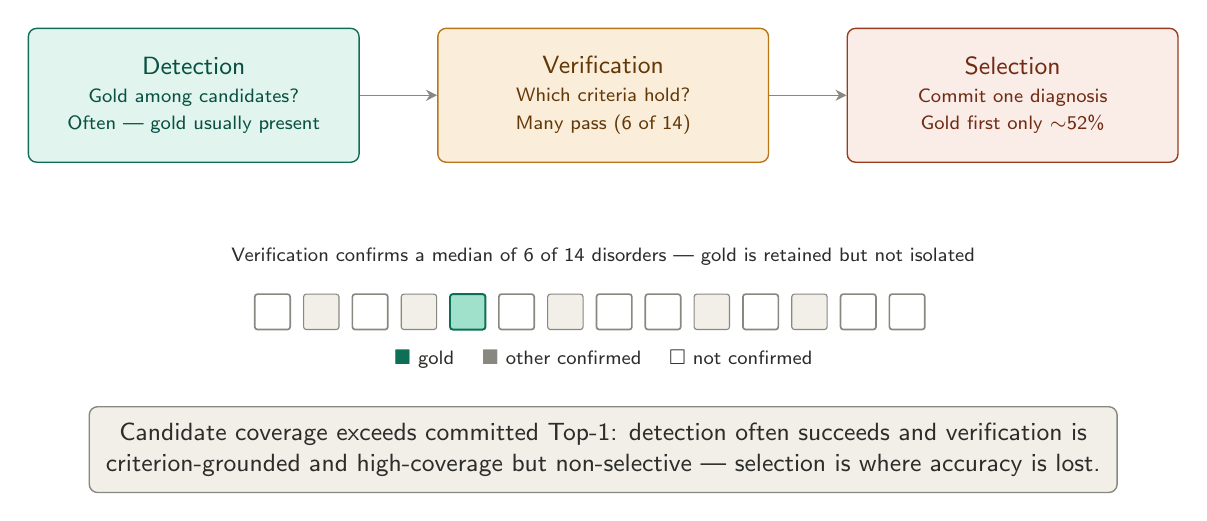
\begin{tikzpicture}[
  font=\small,
  stage/.style={rectangle, rounded corners=3pt, draw, line width=0.5pt, align=center,
                inner sep=4pt, minimum height=17mm, minimum width=42mm},
  det/.style={stage, fill=tealFill, draw=tealDraw, text=tealText},
  ver/.style={stage, fill=ambFill,  draw=ambDraw,  text=ambText},
  sel/.style={stage, fill=corFill,  draw=corDraw,  text=corText},
  arr/.style={-{Stealth[length=4pt,width=4pt]}, line width=0.5pt, draw=gry},
  sq/.style={rectangle, rounded corners=1pt, minimum width=4.5mm, minimum height=4.5mm, inner sep=0pt},
  conf/.style={sq, fill=gryFill, draw=gry, line width=0.4pt},
  outl/.style={sq, fill=none, draw=gry, line width=0.6pt},
  gold/.style={sq, fill=goldFill, draw=goldDraw, line width=0.7pt},
]

% ---- Three stages ----
\node[det] (det) at (0,0)
   {Detection\\[-1pt]{\scriptsize Gold among candidates?}\\[-1pt]{\scriptsize Often --- gold usually present}};
\node[ver] (ver) at (5.2,0)
   {Verification\\[-1pt]{\scriptsize Which criteria hold?}\\[-1pt]{\scriptsize Many pass (6 of 14)}};
\node[sel] (sel) at (10.4,0)
   {Selection\\[-1pt]{\scriptsize Commit one diagnosis}\\[-1pt]{\scriptsize Gold first only $\sim$52\%}};

\draw[arr] (det) -- (ver);
\draw[arr] (ver) -- (sel);

% ---- 14-disorder strip (verification non-selectivity) ----
\node[font=\scriptsize, text=txt] at (5.2,-2.05)
   {Verification confirms a median of 6 of 14 disorders --- gold is retained but not isolated};

% confirmed (gray): indices 1,3,6,9,11 ; gold: 4 ; rest outline
\foreach \i in {0,2,5,7,8,10,12,13}{ \node[outl] at ({1.0+\i*0.62},-2.75) {}; }
\foreach \i in {1,3,6,9,11}{        \node[conf] at ({1.0+\i*0.62},-2.75) {}; }
\node[gold] at ({1.0+4*0.62},-2.75) {};

\node[font=\scriptsize, text=txt] at (5.2,-3.35)
   {\textcolor{goldDraw}{$\blacksquare$} gold \quad \textcolor{gry}{$\blacksquare$} other confirmed \quad $\square$ not confirmed};

% ---- Takeaway ----
\node[rectangle, rounded corners=3pt, draw=gry, line width=0.5pt, fill=gryFill,
      align=center, inner sep=6pt, text=txt, minimum width=128mm] at (5.2,-4.5)
   {Candidate coverage exceeds committed Top-1: detection often succeeds and verification is\\
    criterion-grounded and high-coverage but non-selective --- selection is where accuracy is lost.};

\end{tikzpicture}
\end{document}
